%%%%%%%%%%%%%%%%%%%%%%%%%%%%%%%%%%%%%%%%%%%%%%%%%%%%
%\graphicspath{chapters/figures/}
\chapter{Control Unit}
\label{chap_cu}

%%%%%%%%%%%%%%%%%%%%%%%%%%%%%%%%%%%%%%%%%%%%%%%%%%%%%%%%%%%
\section{Overview}
The Control Unit is the brain of the processor as it needs to command and
coordinate all other functional units. It generally receives from the 
instruction fetch the fields necessary to identify the current instruction and
decides how all other components should behave for the following pipeline
stages. Due to its key role inside the DLX we have carefully considered all
three available options:
\begin{itemize}
	\item \textit{Microprogrammed Control Unit}, is flexible and can be 
		  easily modified to accomodate new instructions. Due to the use of 
		  memory element and the internal program counter it is slower compared 
		  to the other solutions
	\item \textit{Hardwired Control Unit}, is less flexible and still needs a
		  memory element (Lookup Table), but it is faster than the previous
		  solution
	\item \textit{Finite State Machine Control Unit}, is comparable to the
	      hardwired in terms of flexibility but it can be easier to manage
	      and does not need any memory component       
\end{itemize}
\begin{figure}[h]
	\centering
		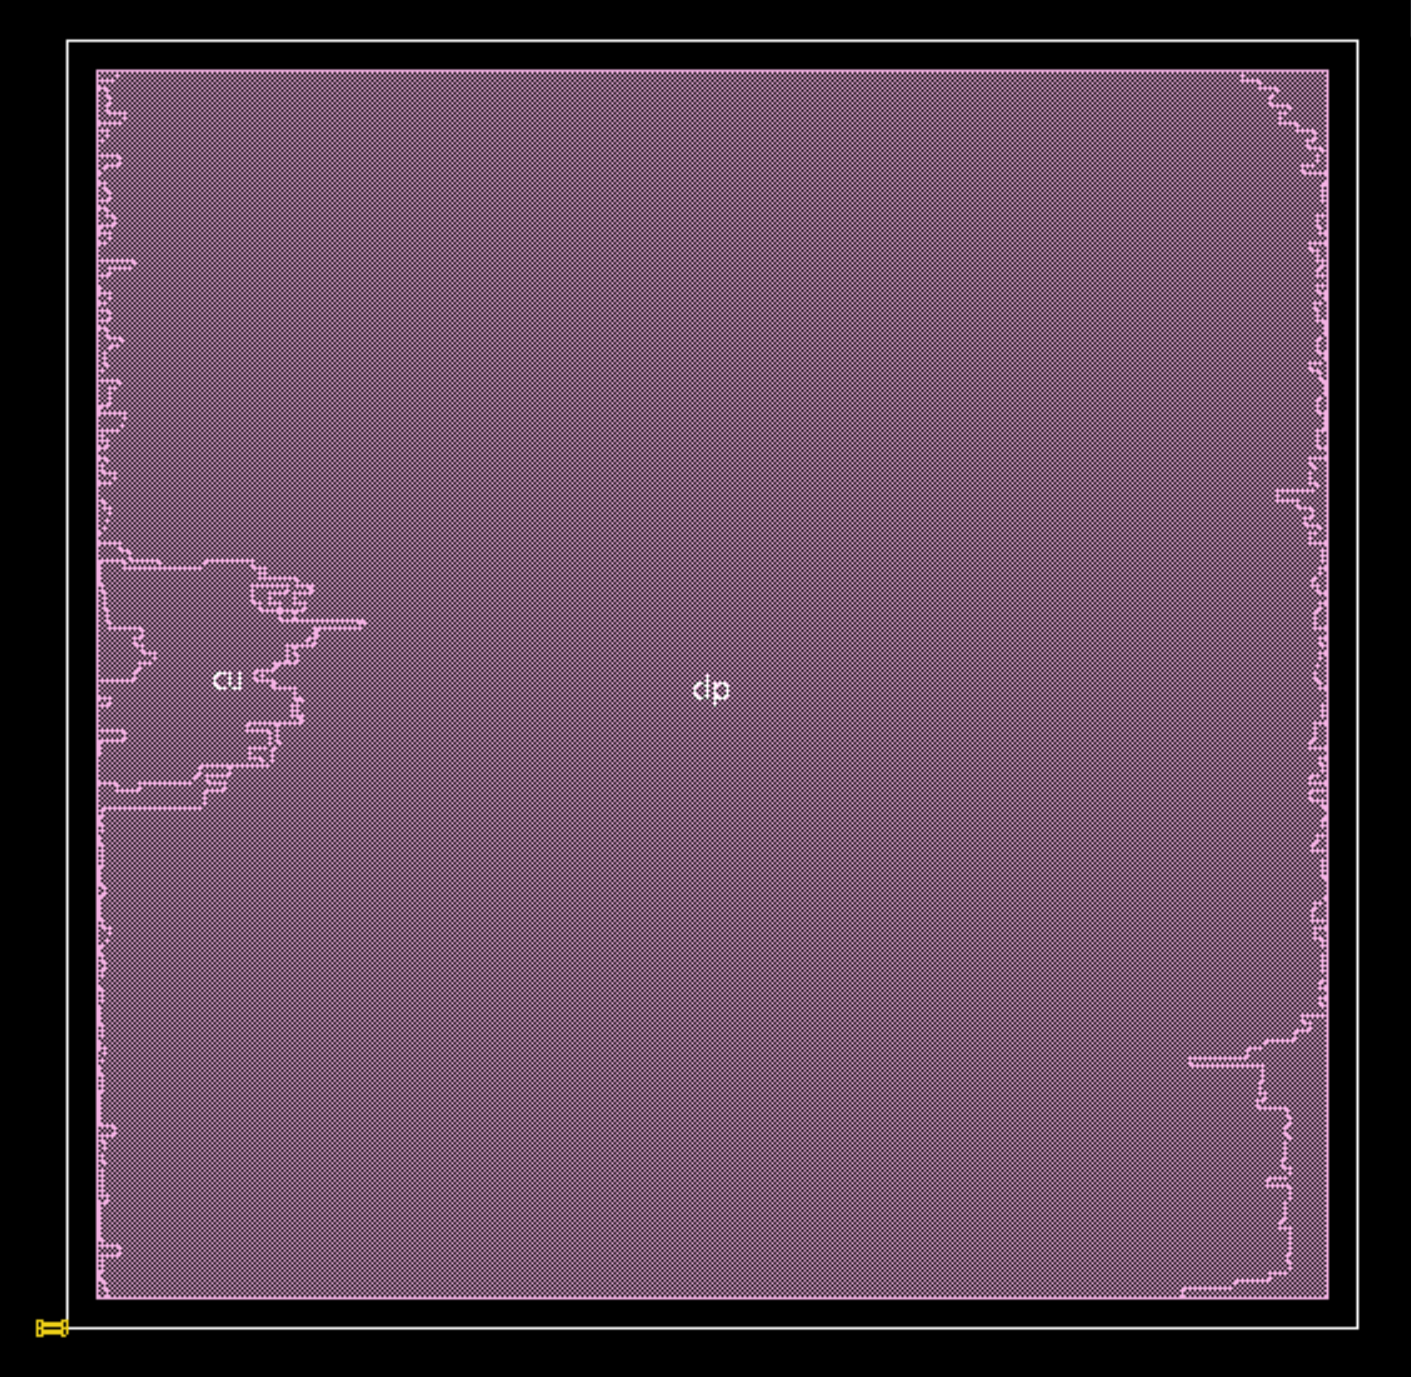
\includegraphics[trim={0.65cm 0.45cm 0.48cm 
		0.37cm},clip=true,scale=0.8]{./Partition_DLX}
	\caption{Amoeba View for the physical layout of the DLX}
	\label{fig:aomeba_view}	
\end{figure}
Our choice verted on the FSM as it is lightweight and fast, moreover by choosing
a Melay type FSM we can further reduce the number of states and thus the area.
We can show the final result in figure ~\ref{fig:aomeba_view} through the 
\textit{amoeba view} feature of Innovus. As a rough estimate the Control Unit 
occupy only $4 \%$ of the total area.

\section{Development}
The first version was quite cumbersome, but easy to follow at its core. The idea
consists in having five identical FSM, composed of five states 
for normal operations and five states for stalling the pipeline. Each FSM
covers a different stage of the pipeline and generates only the control signals
related to that stage, setting the remaining bits of its own control word to
zero. The final control word is then generated by the logical \textit{or} of 
the five control word. This implementation is quite human friendly and simple 
to manage since the conditions for stalling, or generating any abnormal 
behaviour of the pipeline can be determined writing by hand the execution 
of the various stage like in figure ADD FIGURE.
The next version was a small but still meaningful update, due to the removal 
of all enable signals related to the registers between the pipeline stages.
This choice derives from the rare use of those signals and brought a reduction
in the control word size by three bits.
The last update brought major improvements, especially on the size.
Instead of having five FSM managing one part of the pipeline there is now only 
one FSM, with three states, which generates during the instruction fetch the 
full control word. Each control signal is then delayed, using registers, in 
order to hit the target unit at the right time. 

\section{Description} 
The final version is composed of the following states:

\begin{itemize}
	\item \textbf{reset}, is used at boot or during the reset of the system 
	\item \textbf{fetch}, is related to normal operation of the pipeline,
	      indicates that the current instruction can go past the fetch stage
	\item \textbf{stall\_if}, is used to inject a \textit{nop} operation in the
	      following cycle; in general after jump instruction
\end{itemize} 
It is worth noting that the Control unit can only inject stall, i.e. nop in the
fetch stage, in case a flush of the pipeline is needed due to a branch
misprediction, the BP Unit will directly handle the situation flushing also part
of the pipelined control word. This behaviour shift part of the load off the 
control unit keeping its tasks simple.

\section{Input Output}
\begin{figure}[h]
	\centering
	
\includegraphics[scale=0.5]{chapters/figures/DLX_CU}
	\caption{View of the Control Unit as a component}
	\label{cu_comp}
\end{figure}

Here are briefly described the signals used to make decisions and control
the datapath: 
\begin{itemize}
	\item \textit{CLK}, system clock used to synchronize the transaction of 
	      the FSM
	\item \textit{RST}, asynchronous reset 
	\item \textit{OPCODE}, 6-bit field necessary to identify the instruction
	\item \textit{FUNC}, 11-bit field to differentiate among R-Type insructions
	\item \textit{FLUSH}, inject zero inside the pipelined control signal
	      generating stall
	\item \textit{STALL}, generates a stall in the instruction fetch phase
	\item \textit{JMP}, control the policy for sign extension of the immediate 
		  field of I-Type instructions
	\item \textit{RI}, decides whether the address used during write back is
		  the target or source field of the instruction based on its type
	\item \textit{BR\_TYPE}, control if the datapath should check for equality
		  or dis-equality in a branch instruction, generating then the correct
		  immediate value for the following operation : PC + 4 + imm16
	\item \textit{RD1}, enables signal for register file read port one
	\item \textit{RD2}, enables signal for register file read port two
	\item \textit{US}, interacts with the sign extender changing the policy of 
		  the extension from signed to unsigned
	\item \textit{MUX2\_SEL}, selects between register coming from read port one
		  and PC+4
	\item \textit{MUX2\_SEL}, selects between register coming from read port one
		  and extended immediate value
	\item \textit{UN\_SEL}, selects which unit should propagate its result from 
		  execute to memory stage
	\item \textit{OP\_SEL}, decides the operation during the execution stage
	\item \textit{PC\_SEL}, used to inject the computed address, in the execute
	      stage, as the new program counter
	\item \textit{RW}, enable write signal for the external memory
	\item \textit{D\_TYPE}, decides the type of data retrieved from external
	      memory between byte, half-wird and word
	\item \textit{WR}, enable write signal for the register file
	\item \textit{MEM\_ALU\_SEL}, selects which data is written in the register
	      file between the result of the ALU and the memory output 
	\item \textit{INST\_T\_EX}, indicates to the foreword unit if the current 
	      instruction is of I or R Type
	\item \textit{INST\_EX}, used to detect a stall that started in the
	      instruction fetch, to avoid forewording in such case 
	\item \textit{INST\_MEM}, used to detect a stall that started in the
		  instruction fetch, to avoid forewording in such
		  case 								
\end{itemize}




